\documentclass[11pt, oneside]{article}   	% use "amsart" instead of "article" for AMSLaTeX format
\usepackage{geometry}                		% See geometry.pdf to learn the layout options. There are lots.
\geometry{letterpaper}                   		% ... or a4paper or a5paper or ... 
%\geometry{landscape}                		% Activate for rotated page geometry
%\usepackage[parfill]{parskip}    		% Activate to begin paragraphs with an empty line rather than an indent
\usepackage{graphicx}				% Use pdf, png, jpg, or eps§ with pdflatex; use eps in DVI mode
								% TeX will automatically convert eps --> pdf in pdflatex		
\usepackage{amssymb}
\usepackage{amsmath}
\usepackage{enumitem}
\usepackage{caption}
\usepackage{subcaption}
\usepackage{multirow}
\usepackage{array}
\usepackage{float}
%\usepackage{enumitem}

%SetFont

%SetFonts


\title{Project \#3}
\author{Huiyu Wang\\604--592--364}
\date{}							% Activate to display a given date or no date

\begin{document}
\maketitle

\section{Filters}
On top of the given 17 filters, we add 12 Gabor filters with size of 15 and orientations of 0, 30, 60, 90, 120 and 150. In addition, we add 2 first order gradient filters with different direction than the given ones and a $1\times1$ filter. Totally, we have 32 filters. Fig. 1 shows all of the filters. Note here we use the same filters as in the example to make the result comparable. Adding more filters (e.g. using more sizes and directions of gabor filters) will result in better performance in acceptable time consumption.
\begin{figure}[H]
	\centering
	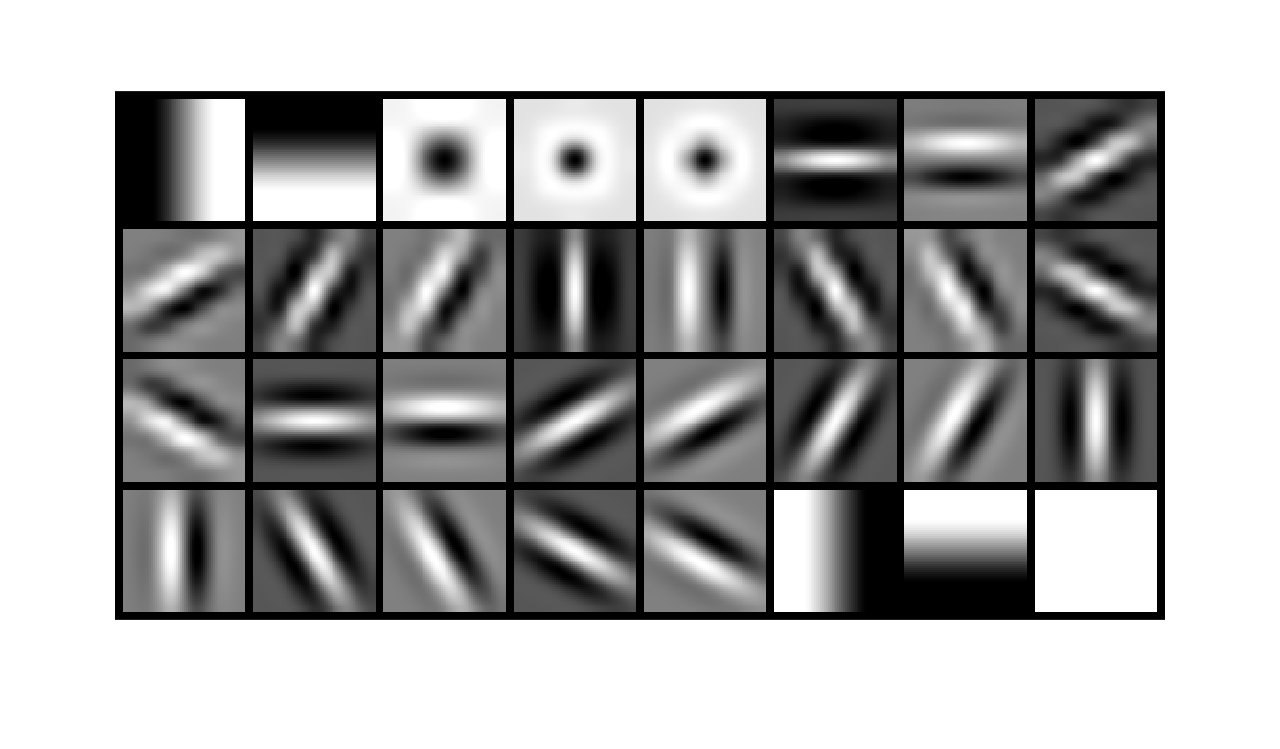
\includegraphics[width=0.8\textwidth]{filters}
	\caption{All of the 32 filters (resized)}
	\label {fig:plot}
\end{figure}

\section{Results}
The initial T is set to be 0.1 and the decreasing coefficient is set to 0.96. Choosing smaller T leads to narrower probability distributions and lower errors. We use 15 bins and assign them with weigthts: [8, 7, 6, 5, 4, 3, 2, 1, 2, 3, 4, 5, 6, 7, 8]. To accelerate the computation, we just consider [0, 7] gray intensity range for each pixel. We also crop and resize the sizes of original images to be $256 \times 256$. The synthesized images are also of size $256 \times 256$ and gray intensity range [0, 7].

\subsection{Fur}
The result using 24 filters out of all 32 filters is good enough (the weighted error is not decreasing). The chosen filters are 3, 20, 2, 12, 1, 32, 6, 31, 22, 30, 27, 16, 8, 26, 4, 19, 28, 29, 23, 10, 14, 24, 25, 21. Figure \ref{fig:fur} shows the curve of the average weighted error per bin over the number of filters used for synthesis. Figure \ref{fig:furs} shows the original image (of size $256 \times 256$ and gray intensity range [0, 7]) and the synthesized images.

\begin{figure}[H]
	\centering
	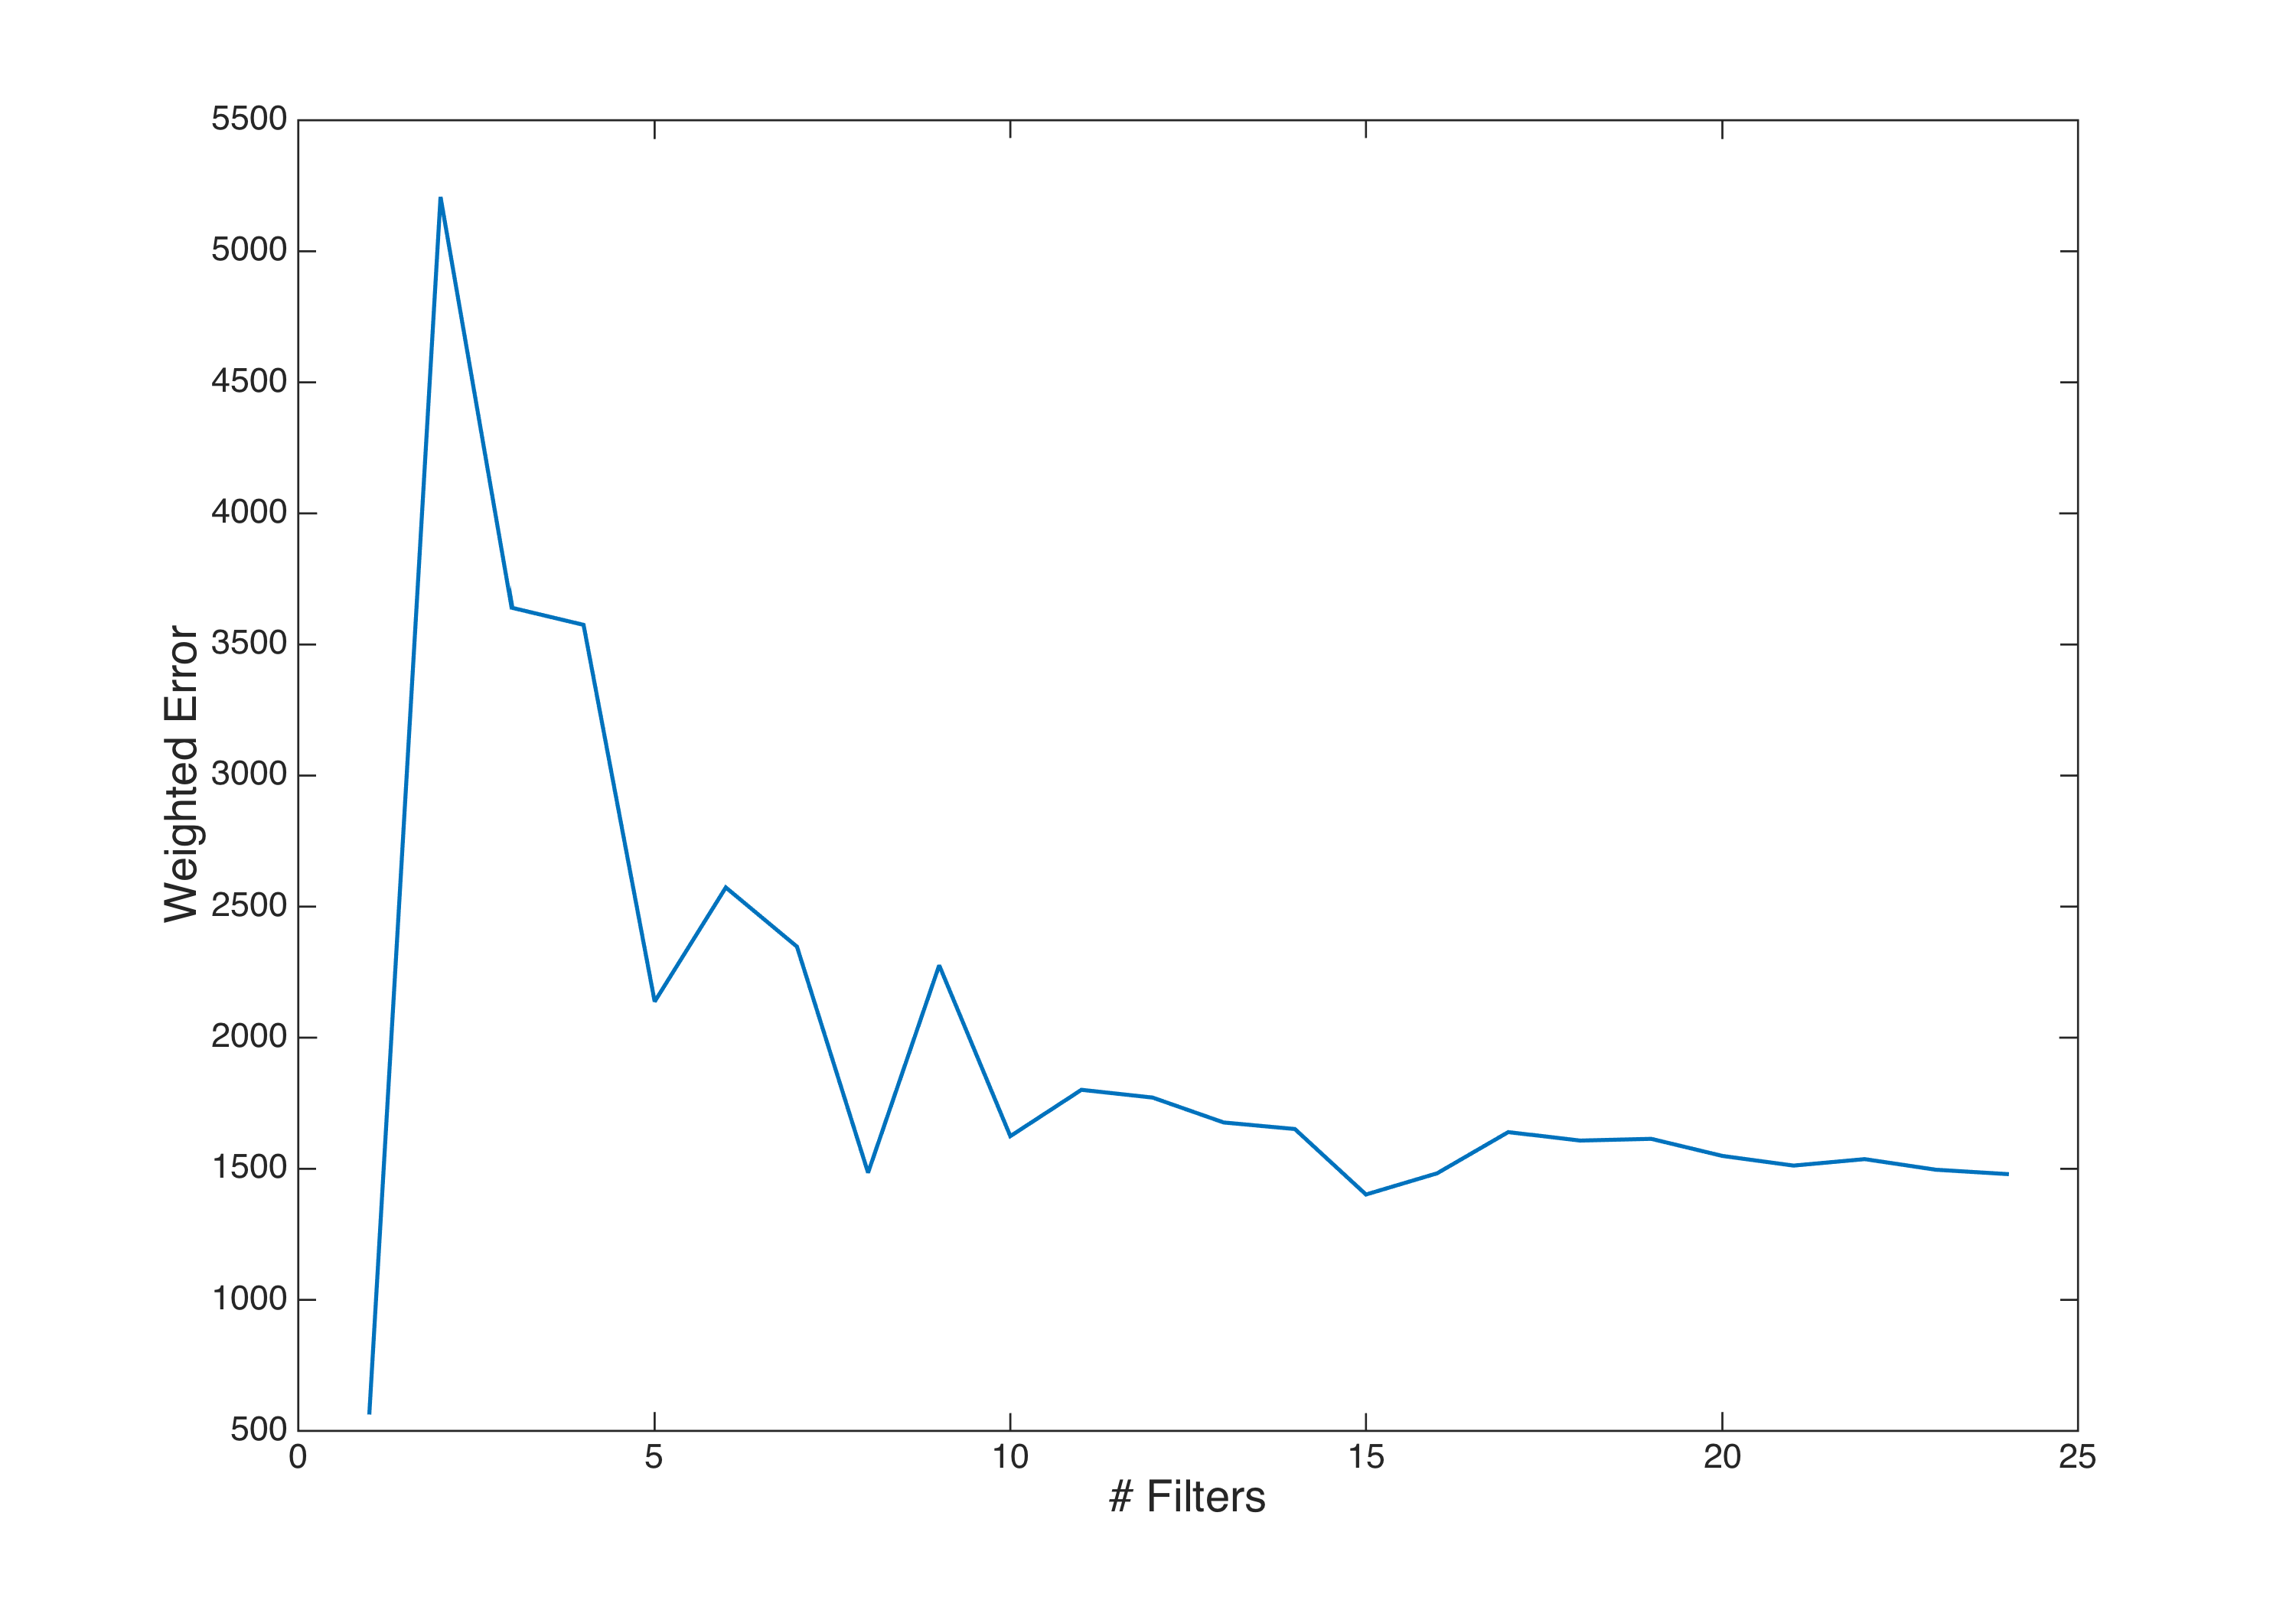
\includegraphics[width=0.9\textwidth]{fur}
	\caption{Error over the number of filters used (fur)}
	\label {fig:fur}
\end{figure}

\begin{figure}[H]
    \centering
    \begin{subfigure}[b]{0.3\textwidth}
        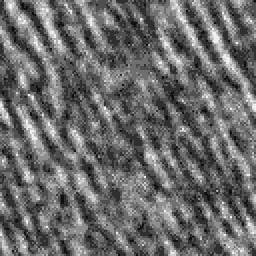
\includegraphics[width=\textwidth]{fur0}
        \caption{Original}
        \label{fig:fur0}
    \end{subfigure}
    \begin{subfigure}[b]{0.3\textwidth}
        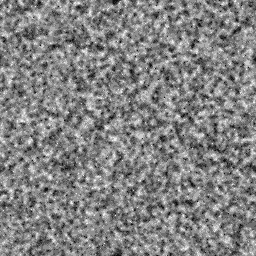
\includegraphics[width=\textwidth]{fur1}
        \caption{1 filter}
        \label{fig:fur1}
    \end{subfigure}
    \begin{subfigure}[b]{0.3\textwidth}
        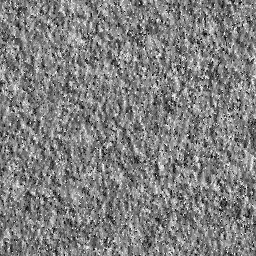
\includegraphics[width=\textwidth]{fur3}
        \caption{3 filters}
        \label{fig:fur3}
    \end{subfigure}
    
    \begin{subfigure}[b]{0.3\textwidth}
        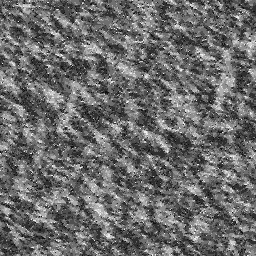
\includegraphics[width=\textwidth]{fur6}
        \caption{6 filters}
        \label{fig:fur6}
    \end{subfigure}
    \begin{subfigure}[b]{0.3\textwidth}
        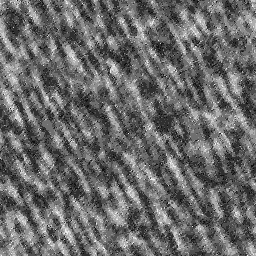
\includegraphics[width=\textwidth]{fur12}
        \caption{12 filters}
        \label{fig:fur12}
    \end{subfigure}
    \begin{subfigure}[b]{0.3\textwidth}
        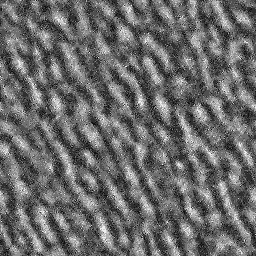
\includegraphics[width=\textwidth]{fur24}
        \caption{24 filters}
        \label{fig:fur24}
    \end{subfigure}
    \caption{Synthesized Images (fur)}\label{fig:furs}
\end{figure}

\subsection{Stucco}
The result using 24 filters out of all 32 filters is good enough (the weighted error is not decreasing). The chosen filters are 32, 4, 26, 16, 3, 14, 1, 2, 22, 30, 28, 31, 20, 12, 6, 10, 19, 8, 5, 17, 24, 15, 7, 13, 29. Figure \ref{fig:stucco} shows the curve of the average weighted error per bin over the number of filters used for synthesis. Figure \ref{fig:stuccos} shows the original image (of size $256 \times 256$ and gray intensity range [0, 7]) and the synthesized images.

\begin{figure}[H]
	\centering
	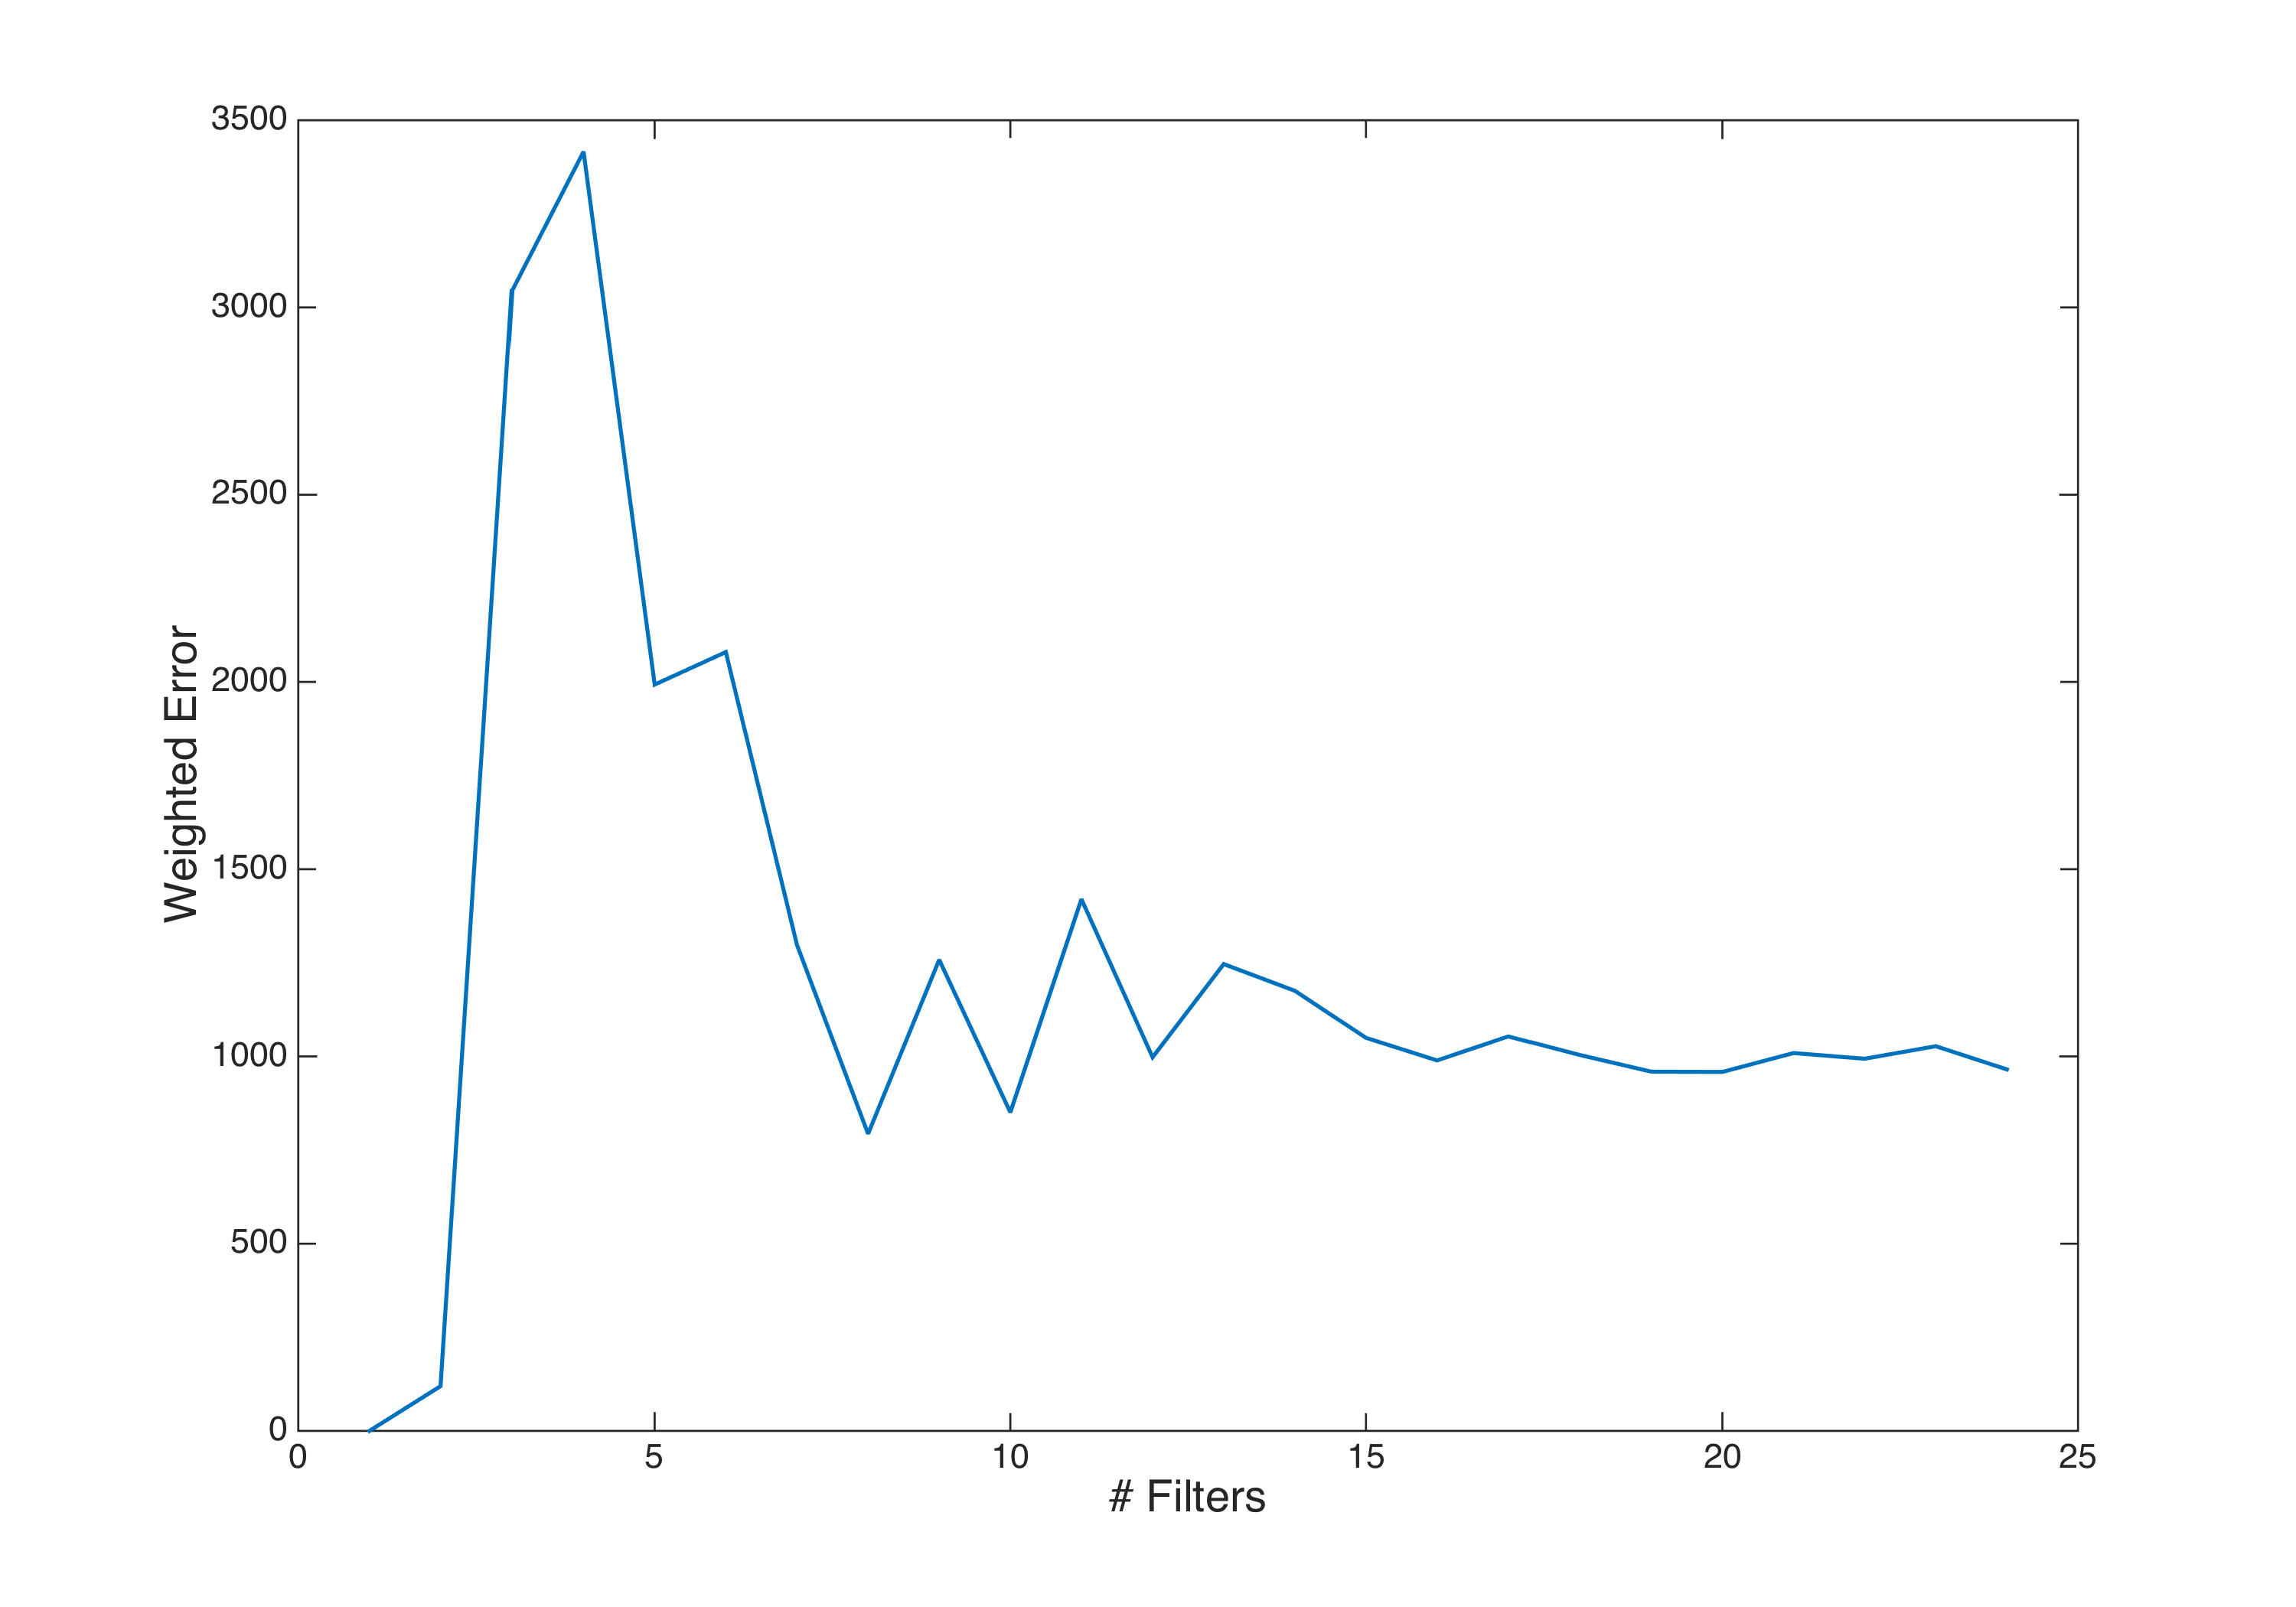
\includegraphics[width=0.9\textwidth]{stucco}
	\caption{Error over the number of filters used (stucco)}
	\label {fig:stucco}
\end{figure}

\begin{figure}[H]
    \centering
    \begin{subfigure}[b]{0.3\textwidth}
        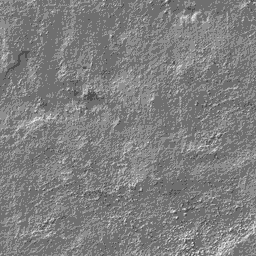
\includegraphics[width=\textwidth]{stucco0}
        \caption{Original}
        \label{fig:stucco0}
    \end{subfigure}
    \begin{subfigure}[b]{0.3\textwidth}
        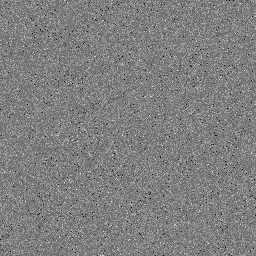
\includegraphics[width=\textwidth]{stucco1}
        \caption{1 filter}
        \label{fig:stucco1}
    \end{subfigure}
    \begin{subfigure}[b]{0.3\textwidth}
        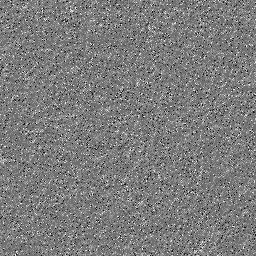
\includegraphics[width=\textwidth]{stucco3}
        \caption{3 filters}
        \label{fig:stucco3}
    \end{subfigure}
    
    \begin{subfigure}[b]{0.3\textwidth}
        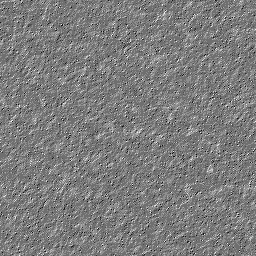
\includegraphics[width=\textwidth]{stucco6}
        \caption{6 filters}
        \label{fig:stucco6}
    \end{subfigure}
    \begin{subfigure}[b]{0.3\textwidth}
        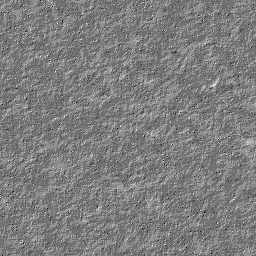
\includegraphics[width=\textwidth]{stucco12}
        \caption{12 filters}
        \label{fig:stucco12}
    \end{subfigure}
    \begin{subfigure}[b]{0.3\textwidth}
        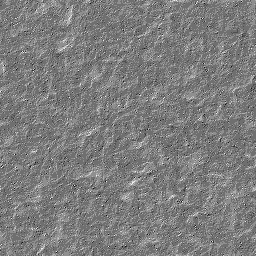
\includegraphics[width=\textwidth]{stucco24}
        \caption{24 filters}
        \label{fig:stucco24}
    \end{subfigure}
    \caption{Synthesized Images (stucco)}\label{fig:stuccos}
\end{figure}

\subsection{Grass}
The result using 24 filters out of all 32 filters is good enough (the weighted error is not decreasing). The chosen filters are 3, 32, 19, 6, 2, 5, 10, 30, 8, 16, 4, 12, 31, 25, 27, 14, 23, 26, 1, 22, 21, 13, 11, 9. Figure \ref{fig:grass} shows the curve of the average weighted error per bin over the number of filters used for synthesis. Figure \ref{fig:grasss} shows the original image (of size $256 \times 256$ and gray intensity range [0, 7]) and the synthesized images.

\begin{figure}[H]
	\centering
	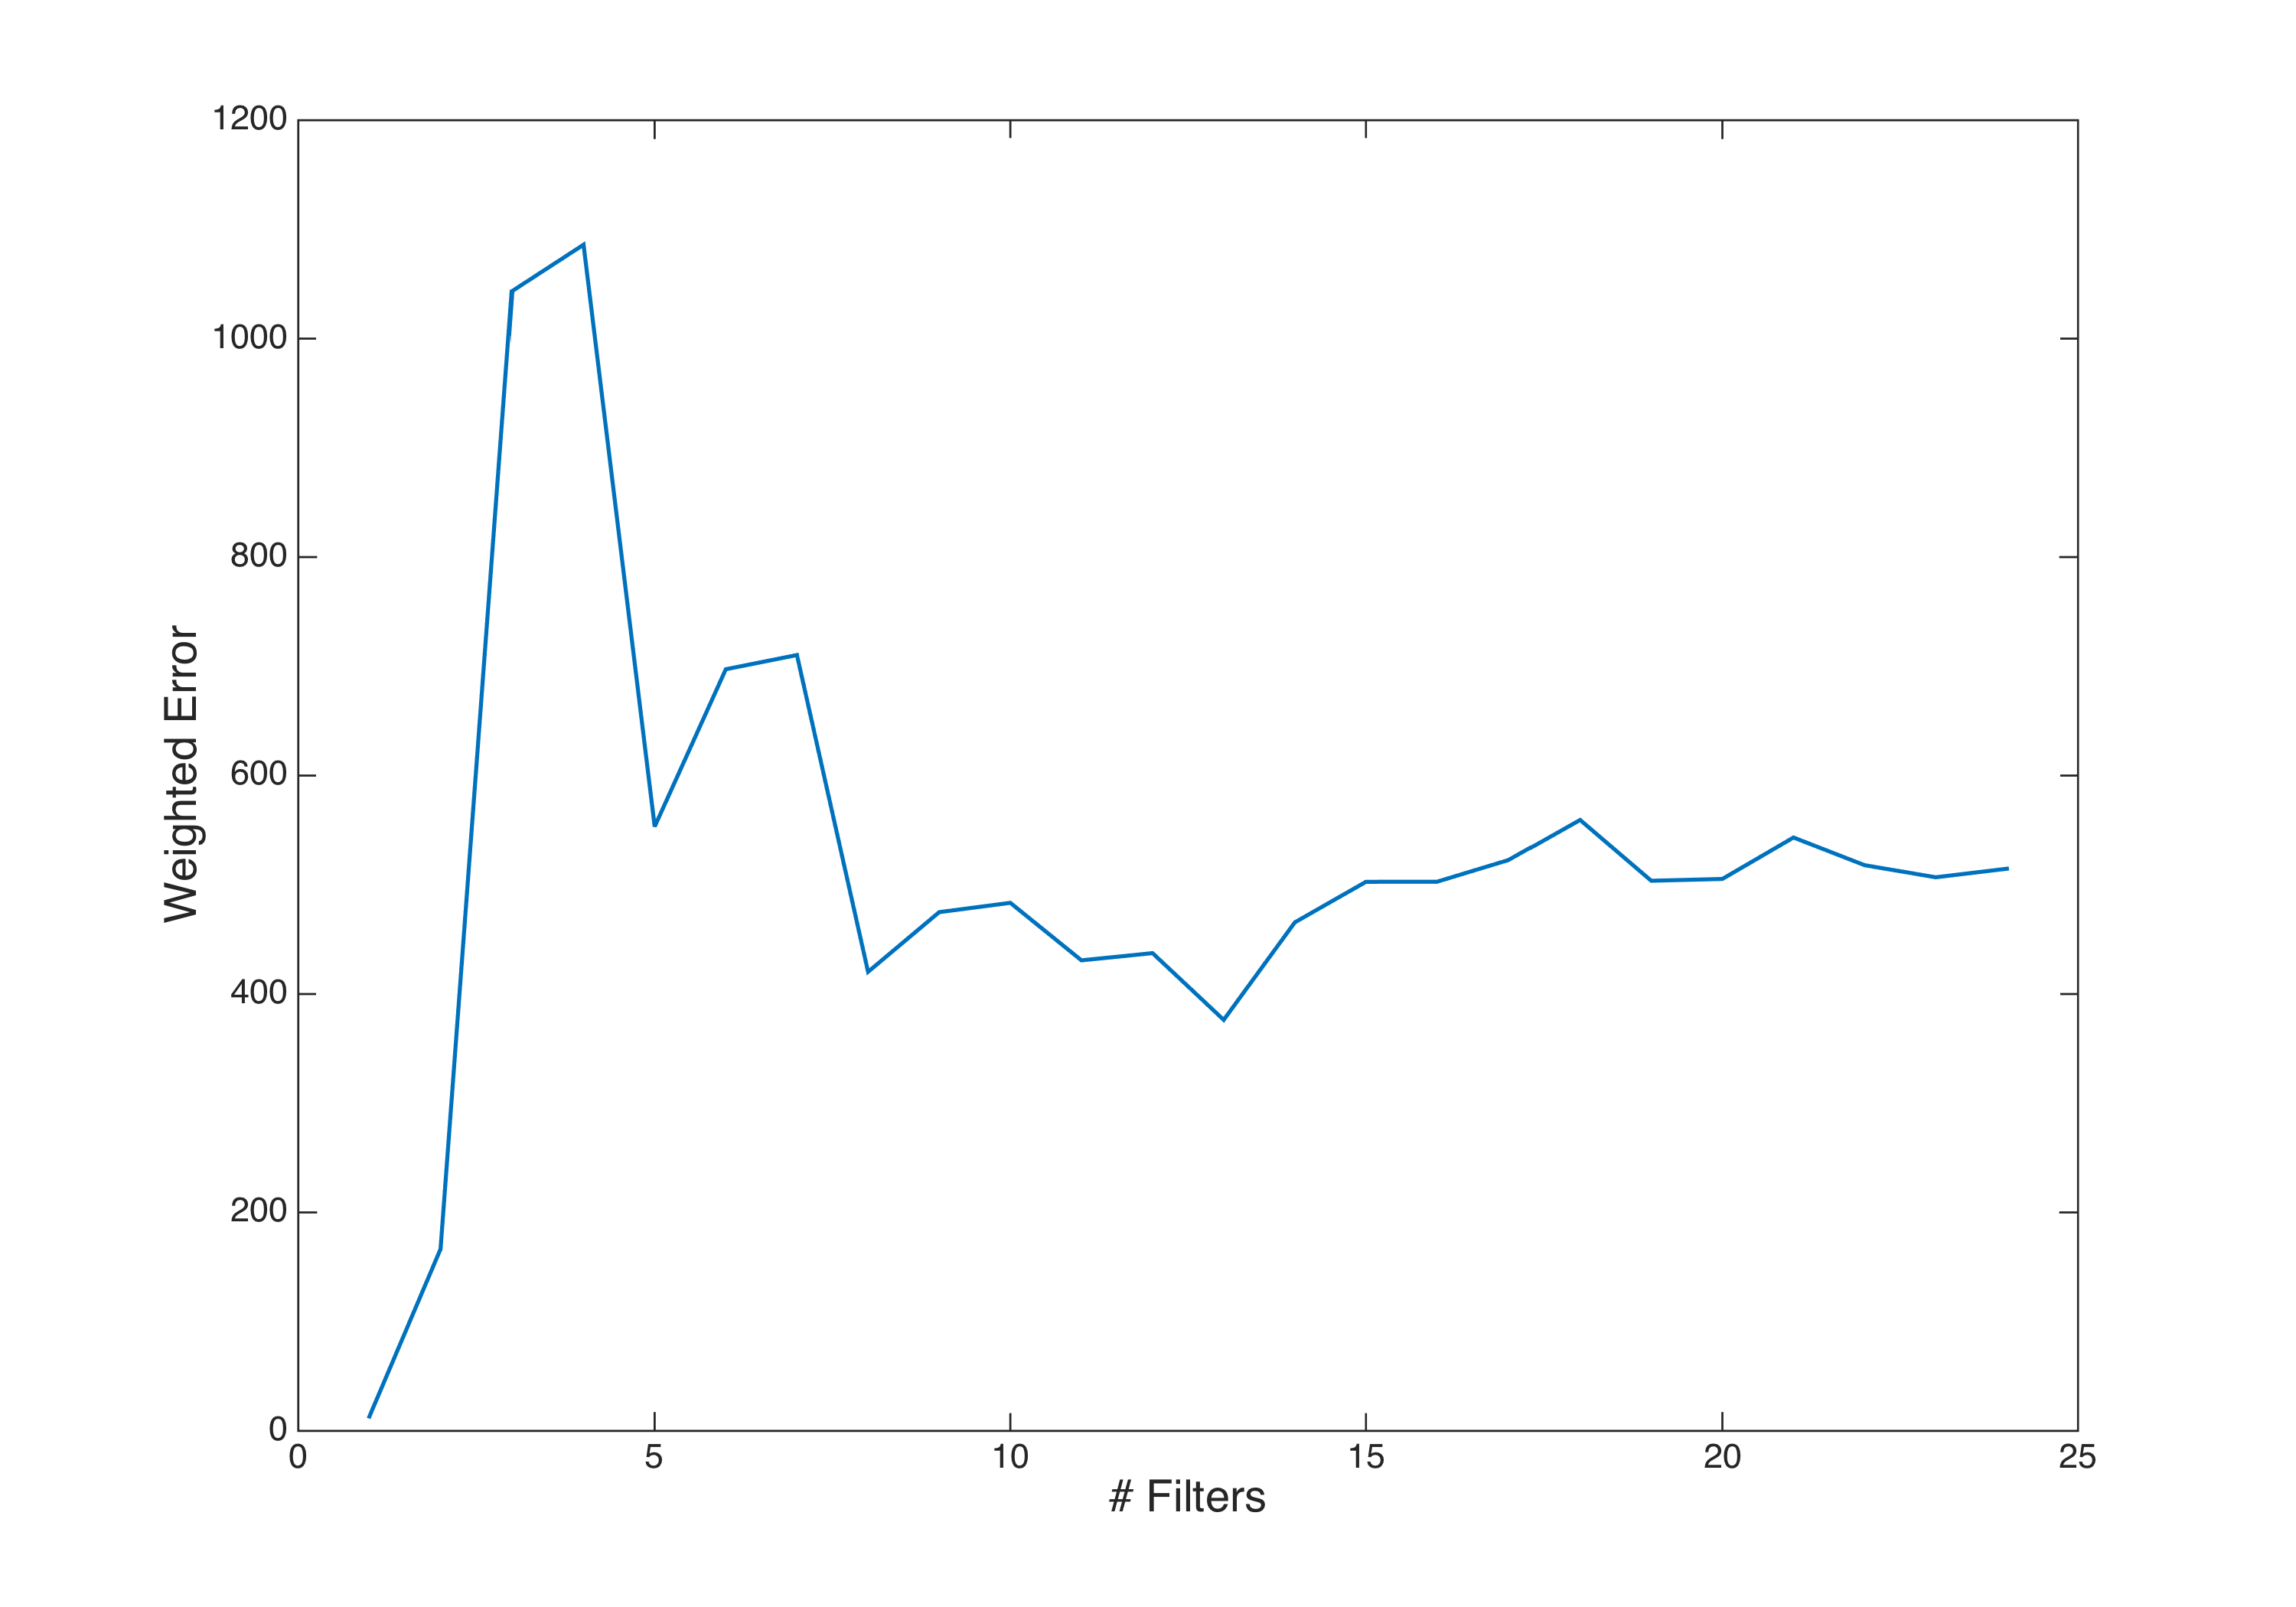
\includegraphics[width=0.9\textwidth]{grass}
	\caption{Error over the number of filters used (grass)}
	\label {fig:grass}
\end{figure}

\begin{figure}[H]
    \centering
    \begin{subfigure}[b]{0.3\textwidth}
        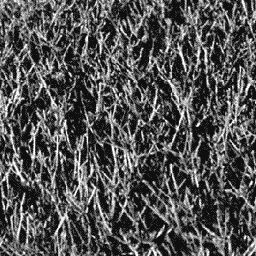
\includegraphics[width=\textwidth]{grass0}
        \caption{Original}
        \label{fig:grass0}
    \end{subfigure}
    \begin{subfigure}[b]{0.3\textwidth}
        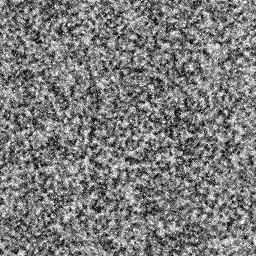
\includegraphics[width=\textwidth]{grass1}
        \caption{1 filter}
        \label{fig:grass1}
    \end{subfigure}
    \begin{subfigure}[b]{0.3\textwidth}
        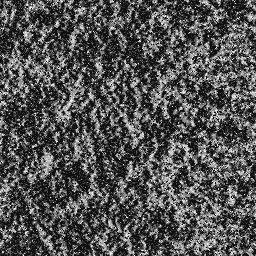
\includegraphics[width=\textwidth]{grass3}
        \caption{3 filters}
        \label{fig:grass3}
    \end{subfigure}
    
    \begin{subfigure}[b]{0.3\textwidth}
        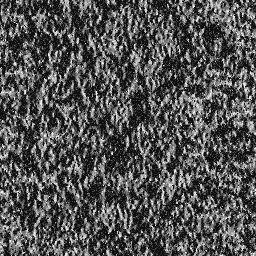
\includegraphics[width=\textwidth]{grass6}
        \caption{6 filters}
        \label{fig:grass6}
    \end{subfigure}
    \begin{subfigure}[b]{0.3\textwidth}
        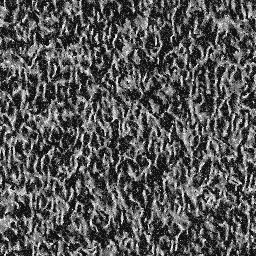
\includegraphics[width=\textwidth]{grass12}
        \caption{12 filters}
        \label{fig:grass12}
    \end{subfigure}
    \begin{subfigure}[b]{0.3\textwidth}
        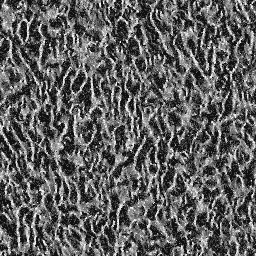
\includegraphics[width=\textwidth]{grass24}
        \caption{24 filters}
        \label{fig:grass24}
    \end{subfigure}
    \caption{Synthesized Images (grass)}\label{fig:grasss}
\end{figure}

\end{document}  